\section{Progress and Timeline}
\subsection[Progress]{Current Progress}

\frame{
	\frametitle{Progress - Coursework}
	\scriptsize
	\begin{table}[!htbp]
		\centering	
  		\begin{tabular}{@{}p{0.6\textwidth} r r@{}}
		\toprule
		\multicolumn{3}{c}{\textbf{Coursework}}\\
		\midrule
		\multicolumn{1}{c}{\textbf{Item}} & \multicolumn{1}{c}{\textbf{Timeline}} & \multicolumn{1}{c}{\textbf{Status}}\\
		\midrule
		MCSC-6010G: Mathematical Modelling & Sep. - Dec. 2018 & Complete\\
		MCSC-6030G: High Performance Computing & Sep. - Dec. 2018 & Complete\\
		NUCL-6005G: Computational Thermodynamics [PhD level elective] & Sep. - Dec. 2018 & Complete\\
		MCSC-6020G: Numerical Analysis & Sep. - Dec. 2019 & Complete\\
		\bottomrule
      		\end{tabular}
	\end{table}
}

\frame{
	\frametitle{Progress - Publications}
	\footnotesize
	\begin{enumerate}{
		\item {M.\ Piro}, {M.\ Poschmann} and \textbf{P.\ Bajpai}, \textit{On the interpretation of chemical potentials computed from equilibrium thermodynamic codes: Applications to molten salts}, \href{https://doi.org/10.1016/j.jnucmat.2019.151756}{Journal of Nuclear Materials, 526 (2019) 151756}.
		\item \textbf{P.\ Bajpai}, {M.\ Poschmann}, {M.\ Piro}, \textit{Derivations of useful partial molar excess Gibbs energy of mixing expressions of common thermodynamic models}, To be submitted to \href{https://www.journals.elsevier.com/calphad}{CALPHAD Computer Coupling of Phase Diagrams and Thermochemistry}. [In preparation]
		\item \textbf{P.\ Bajpai}, {M.\ Poschmann}, {D.\ Andr\v{s}}, {C.\ Bhave}, {M.\ Tonks} and {M.\ Piro}, \textit{Development of a new thermochemistry solver for multiphysics simulations of nuclear materials}, \href{http://https://www.tms.org/TMS2020}{TMS 2020 Supplemental Proceedings, TMS 2020  - 149\textsuperscript{th} Annual Meeting \& Exhibition, San Diego, February 23-27, 2020}. [Accepted]
		\item \textbf{P.\ Bajpai}, {M.\ Poschmann}, {D.\ Andr\v{s}} and {M.\ Piro}, \textit{Progress in developing a new thermochemistry code for corrosion modelling and multiphysics simulation of nuclear fuels}, \href{http://cns-annual-conference.org/2019/index.html}{39\textsuperscript{th} Annual Conference of the Canadian Nuclear Society and 43\textsuperscript{rd} Annual CNS/CNA Student Conference, Ottawa, June 23-26, 2019}.
	}
	\end{enumerate}	
}

\frame{
	\frametitle{Progress - Research}
	\begin{figure}[htbp]
		\begin{center}
		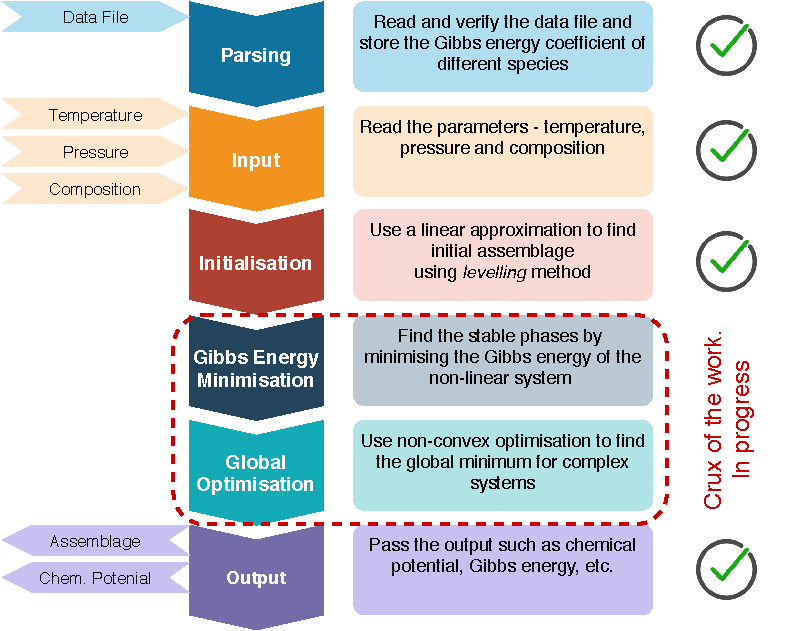
\includegraphics[height=0.65\paperheight]{Figures/YJ_Progress.pdf}
		\end{center}
	\end{figure}
}

\frame{
	\frametitle{Demonstration Problem}
	\only<1>{
	\begin{itemize}
	\item<1> Initial focus on Ni alloys interacting with molten \ce{LiF2 - KF} salts.
	\end{itemize}
	\begin{figure}[htbp]
		\begin{center}
		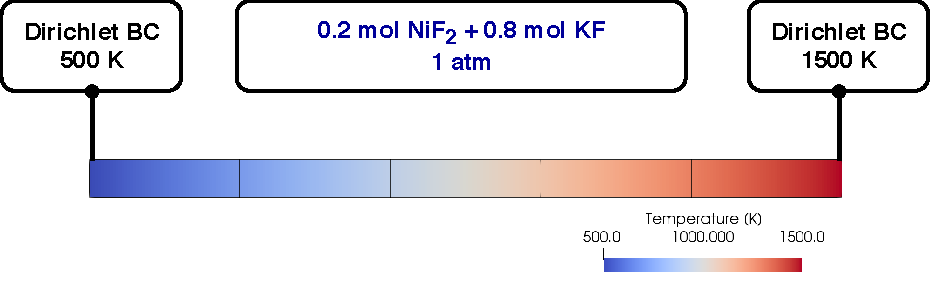
\includegraphics[width=0.85\textwidth]{Figures/Demo_prob.pdf}
		\end{center}
	\end{figure}}
	
	\only<2>{
	\begin{figure}[htbp]
		\begin{center}
		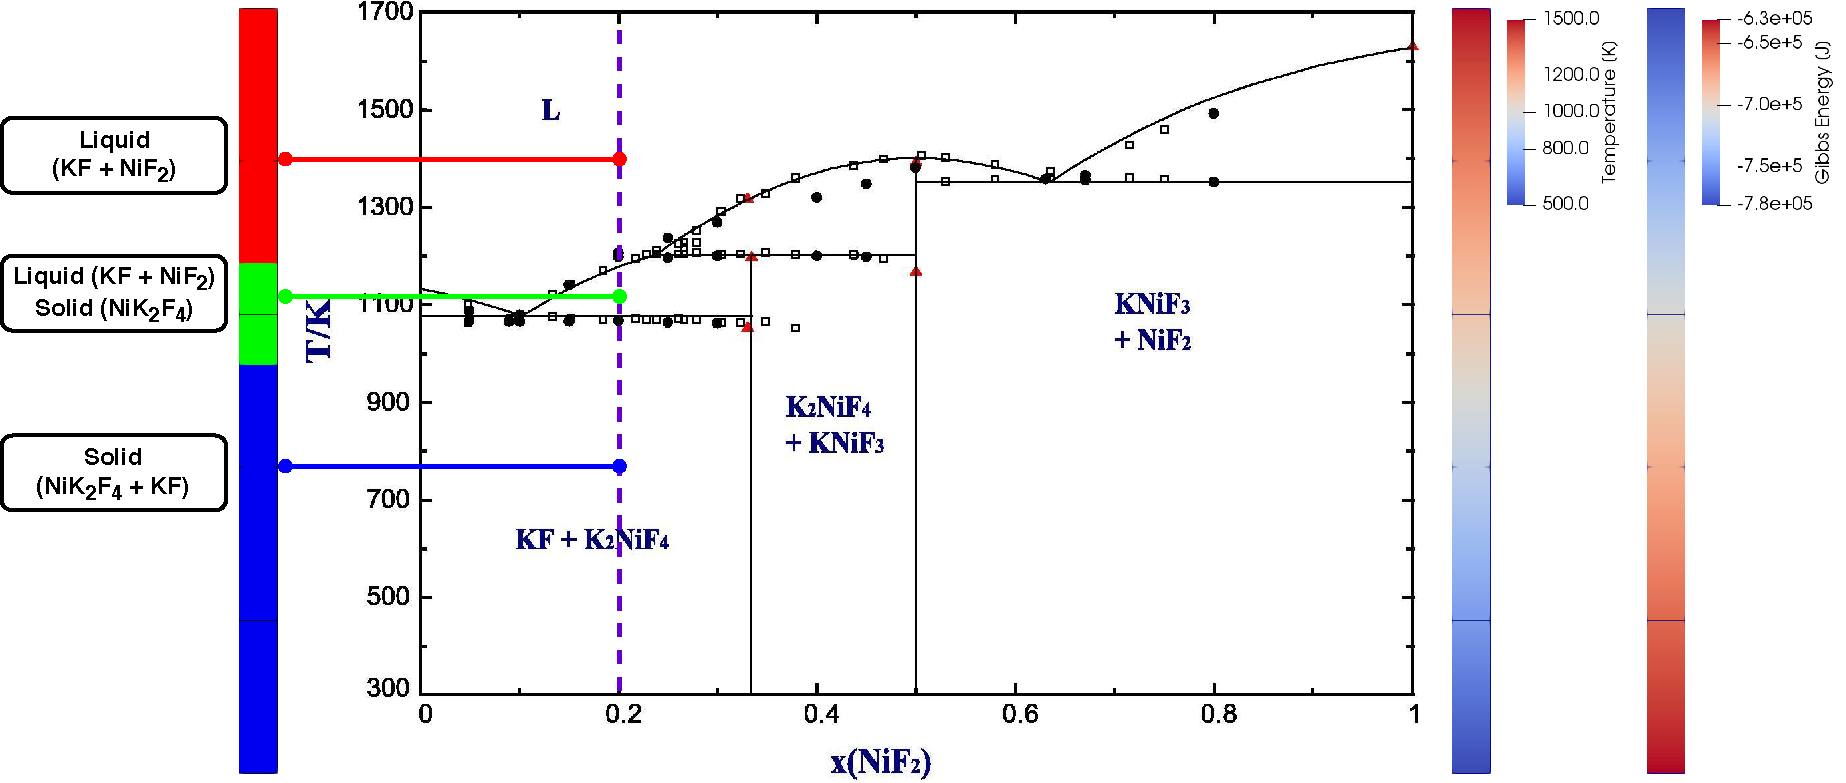
\includegraphics[width=0.85\paperwidth]{Figures/Results.pdf}
		\end{center}
	\end{figure}}
}

\subsection[Milestones]{Milestones}


\frame{
	\frametitle{Milestones - Research}
	\scriptsize
	\begin{table}[!htbp]
		\centering	
  		\begin{tabular}{@{}p{0.6\textwidth} r r@{}}
		\toprule
		\multicolumn{3}{c}{\textbf{Research}}\\
		\midrule
		\multicolumn{1}{c}{\textbf{Item}} & \multicolumn{1}{c}{\textbf{Timeline}} & \multicolumn{1}{c}{\textbf{Status}}\\
		\midrule
		Literature review of computational thermodynamics and GEM & Sep. - Dec. 2018 & Complete\\
		Implement data file parsing code & Feb. - Mar. 2019 & Complete\\
		Implement linear solver (levelling) & Apr. - Jun. 2019 & Complete\\
		Implement communication between Yellowjacket and MOOSE & Jul. - Aug. 2019 & Complete\\
		Implement non-linear solver for GEM (homogeneous) & Sep. - Feb. 2020 & In progress\\
		Implement non-linear solver for GEM (heterogeneous) & Mar. - May 2020 & Planned\\
		Demonstration of non-linear solver capabilities & May - Jun. 2020 & Planned\\
		Begin integration of thermodynamic solver with Marmot & Jul. - Aug. 2020 & Planned\\ 
		Comparative study of global optimisation strategies & Sep. - Dec. 2020 & Planned\\
		Implementation of global optimisation algorithm & Jan. - Mar. 2021 & Planned\\
		Demonstration of global optimisation capabilities & Apr. - May 2021 & Planned\\
		Complete integration into MOOSE & Jun. - Aug. 2021 & Planned\\
		Verification and testing & Sep. - Dec. 2021 & Planned\\
		\bottomrule
      		\end{tabular}
	\end{table}
}